\chapter{Attentive Guidance}\label{Chapter:proposals}

In this chapter I introduce the concept of \textbf{Attentive Guidance (AG)} which is a novel mechanism to equip seq2seq models with an additional bias to nudge them in the direction of finding a compositional solution from the search space of all possible solutions. This chapter begins with a brief overview of the prime motivation for my proposal, followed by the details of attentive guidance. I conclude by showing how attentive guidance relates to the concept of pondering that we saw in section \ref{mtv:ponder}.
%(models capable of zero shot generalizing to unseen inputs on known compositions). Additional these small percentage of models also only showed a weak form of composition wherein if for instance t1, t2 are atomic tables, then a composition task t1 t2 is indexed to prompt t1t2, instead of solving in a nested fashion viz. t1(t2(.)). (Get feedback here, see if this is clear)

\section{Inspiration} 

\cite{Lake2015} introduced Hierarchical Bayesian Program Learning (HBPL) to learn complex characters (concepts) from few samples by representing them as probabilistic programs which are built compositionally via. bayesian sampling from simpler primitives, subparts, parts and the relations between them, respectively. This approach led to human level generalization on the \textbf{omniglot} dataset \citep{Lake2015} which is a dataset containing 1623 characters (concepts) with 20 samples each. Omniglot is therefore not sample intensive and hence ideally suited to test one-shot generalization capabilities of a model. This work served as the major motivation for learning nested functions such as \textit{lookup tables} of the form t1(t2(.), by learning the compositions from simpler primitives i.e. atomic tables and then stacking them hierarchically. The procedure for learning the \textbf{trace} of the above-mentioned task is described subsequently.

\section{Implementation}

Attention (section \ref{mtv:attn}) based seq2seq models produce a \lq soft{}\rq\ alignment between the source (latent representation of the input) and the target. Furthermore seq2seq models require thousands of samples to learn this soft alignment. However in light of the aforementioned arguments presented in favor of concentrating on primitives to construct a complex \lq composition{}\rq\ I propose the concept of \textbf{A}ttentive \textbf{G}uidance (AG). AG argues that the decoder having perfect access to the encoder state(s) containing maximum information pertaining to that decoding step, would leave to improved target sequence accuracy.

\begin{figure}
	\begin{minipage}[t]{\textwidth}
		\ifpdf
		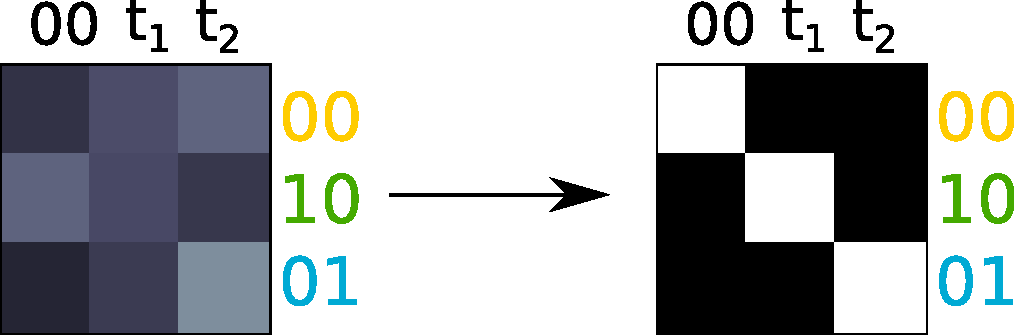
\includegraphics[width=\linewidth,keepaspectratio=true]{./figs/attention-guidance-pdf}
		\else
		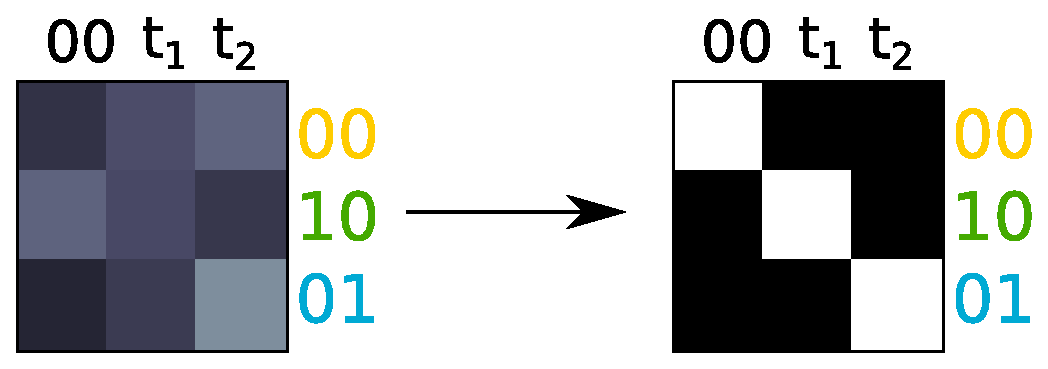
\includegraphics[width=\linewidth,keepaspectratio=true]{./figs/attention-guidance-eps}
		\fi
		\caption{\small Diffused vs Hard Attention}
		\label{pm:ag-schematic}
	\end{minipage}
\end{figure}

Revisiting the query-key-value pair view of attention described in section \ref{mtv:attn}, AG tries to improve the scalar matching score between the query and the keys during the attentive read step. Since the \textit{keys} can be thought of as the memory addresses to the \textit{values} which are needed at a given decoding step, AG tries to ensure a more efficient information retrieval. Similar to \cite{Lake2015} AG induces the trace of a program (albeit not probabilistic) needed to solve a complex composition by solving its subparts in a sequential and hierarchical fashion. This in turn forces the model search for a compositional solution from the space of all possible solutions. AG eventually results in a \lq hard{}\rq\ alignment between the source and target as seen in figure \ref{pm:ag-schematic}


\begin{figure}
	\begin{minipage}[t]{\textwidth}
		\ifpdf
		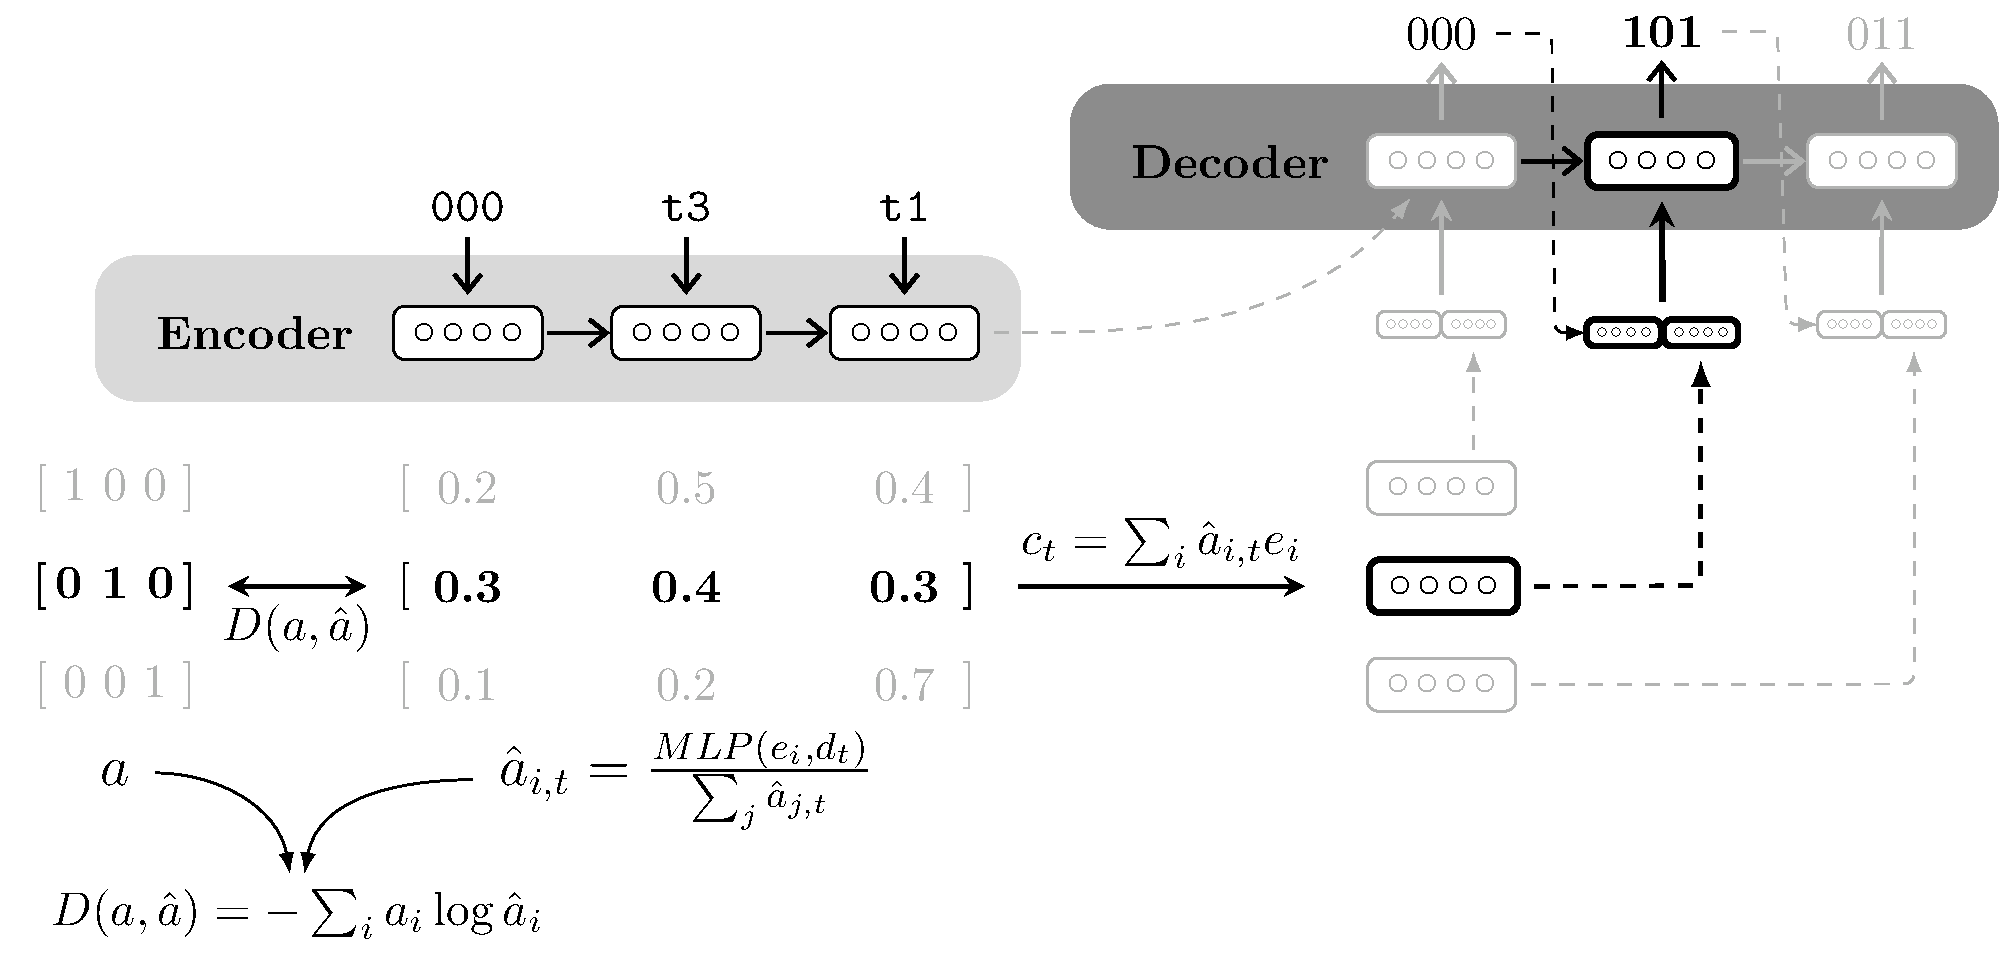
\includegraphics[width=\linewidth,keepaspectratio=true]{./figs/ag-model-pdf}
		\else
		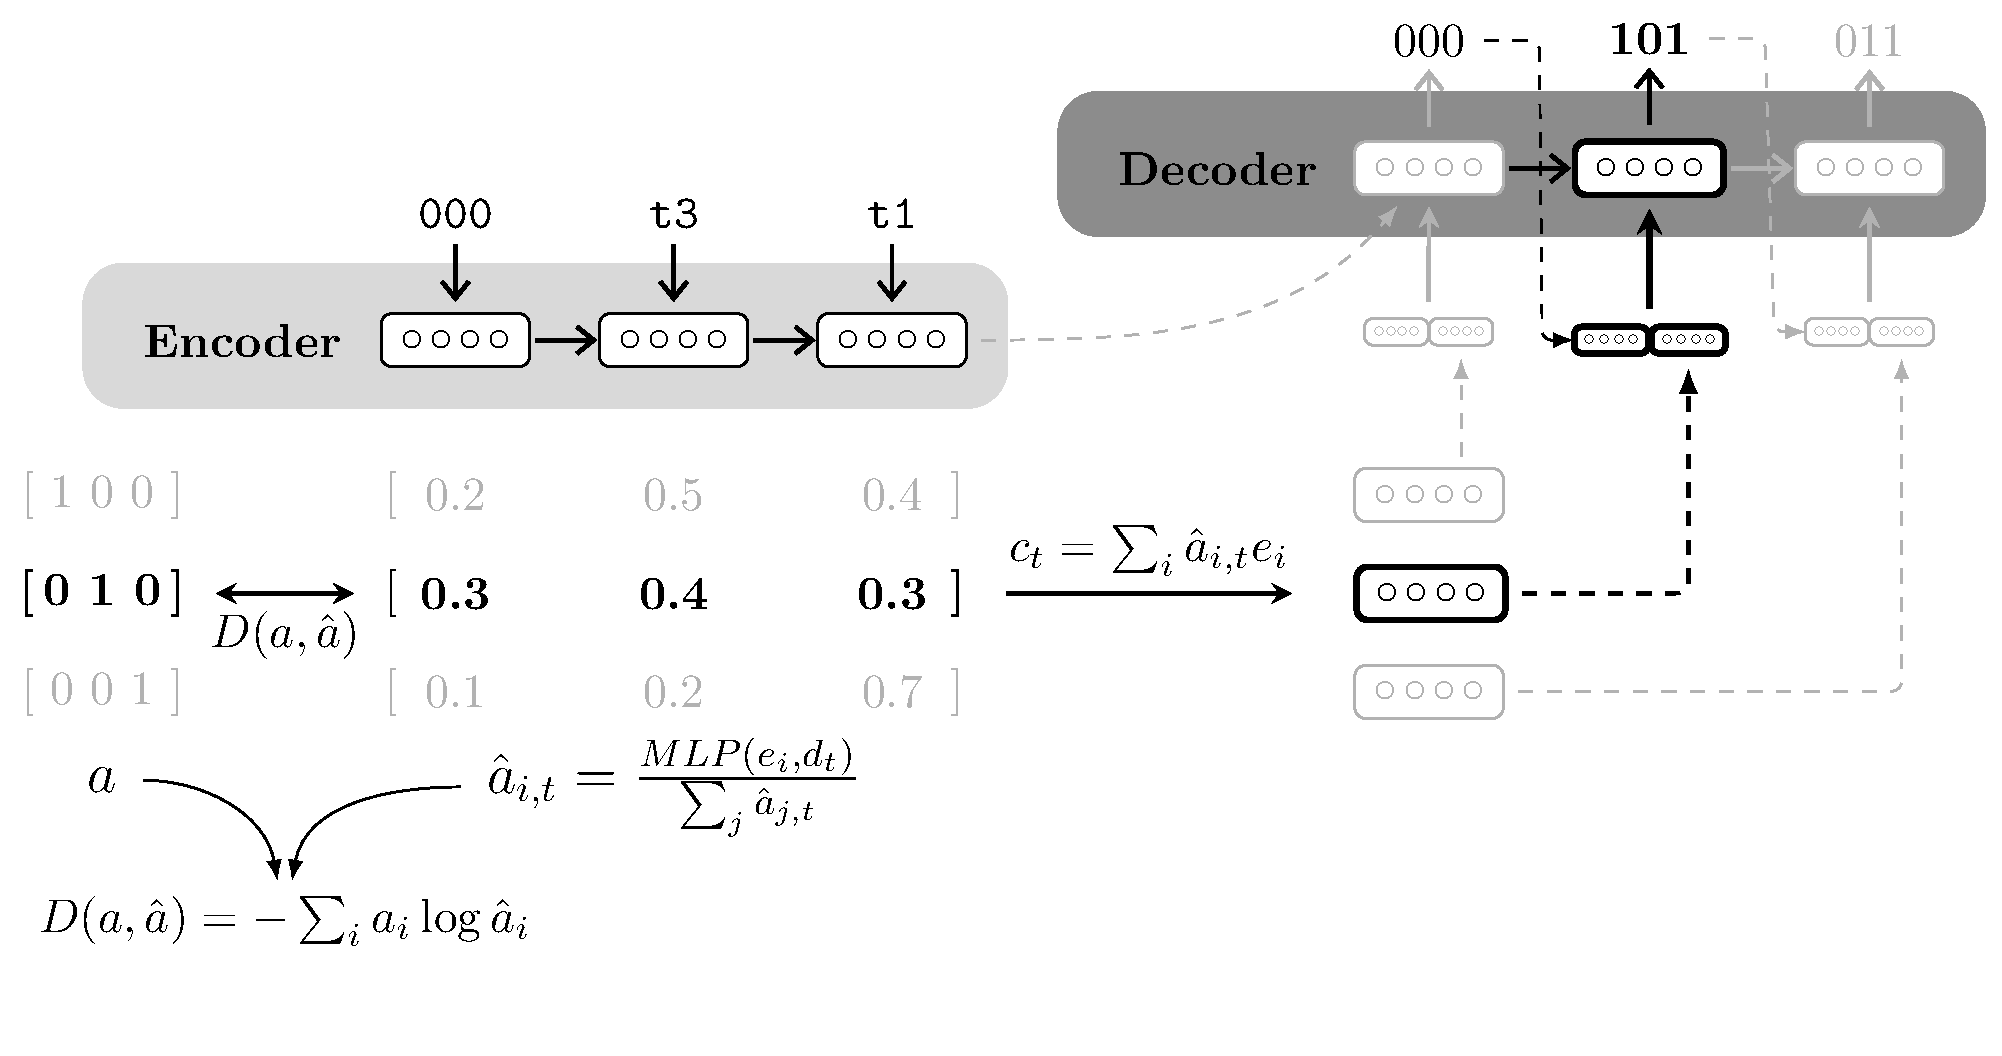
\includegraphics[width=\linewidth,keepaspectratio=true]{./figs/ag-model-eps}
		\fi
		\caption{\small Attentive Guidance and calculation of AG loss \citep{Hupkes2018}}
		\label{pm:ag-loss}
	\end{minipage}
\end{figure}

AG is implemented via an extra loss term added to the final model loss. As shown in figure \ref{pm:ag-loss}, at each step of decoding, the cross entropy loss between calculated attention vector $\hat{a}_{t,i}$ and the ideal attention vector $a_{t,i}$, are added to the model loss. The final loss for an output sequence of length $T$ and an input sequence of length $N$ is therefore expressed as:

\begin{equation}
\widetilde{\mathcal{L}}(x,y) = \mathcal{L}(x,y) + \sum_{t=1}^T \sum_{i=1}^N -a_{i,t}\log\hat{a}_{i,t}
\end{equation}

\section{AG and Pondering} \label{pm:ag-ponder}
Pondering presented in section \ref{mtv:ponder} facilitates variable hidden state transitions at any given input step in a recurrent unit. Attentive guidance can be seen as hardcoded or forced pondering in case of seq2seq models. This is best elaborated through an example as follows:
\begin{equation}
	f(5) = 10 \qquad g(3) = 5\qquad f(g(3)) = 10,
\end{equation}
rewriting the composed function as follows and expanding each step of composition:
\begin{equation}
	f\ g\ 3 = 5\ 10.
\end{equation}
It is easy to see that if the above example is presented to a model all it needs to do is emit the final output i.e. 10. However AG forces an additional (ponder) step to explicitly emit the intermediate output as well. Not only does this allow the decoder of the output to have an additional hidden state transition it also helps us see if the model is taking compositional steps in arriving at the final answer. In this thesis we use such \lq mocked\rq{} pondering in case of lookup-tables (section \ref{datasets:lt}) and micro tasks (chapter \ref{Chapter:datasets}). As a future work we can think about coming up with a method to ensure that the number of ponder steps are learned by the decoder instead of being hardcoded.s